\documentclass[UTF8]{ctexart}
\usepackage{enumerate}
\usepackage{cite}
\usepackage{graphicx}
\usepackage[linesnumbered,boxed]{algorithm2e}
\usepackage{listings}
\usepackage{color}
\begin{document}
\title{关于中断那些事儿}
\author{寇一笑}
\date{\today}
\maketitle
\lstset{frame=tb,
  language=C,
  aboveskip=3mm,
  belowskip=3mm,
  showstringspaces=false,
  columns=flexible,
  basicstyle={\small\ttfamily},
  numbers=none,
  numberstyle=\tiny\color{gray},
  keywordstyle=\color{blue},
  commentstyle=\color{dkgreen},
  stringstyle=\color{mauve},
  breaklines=true,
  breakatwhitespace=true,
  tabsize=3,
  escapeinside=``
}
\begin{abstract}
随着计算机技术的飞速发展,微处理器控制输入/输出部件或者端口的数据传送方式也在不断的进步和发展。现代计算机系统中,都毫不例外地引入了中断系统。本文主要是围绕中断这一主题,从中断的定义到中断的用途、在汇编语言上的使用等方面谈谈我对中断的理解。
\end{abstract}
\section{中断是什么}
中断是计算机中的一个十分重要的概念,在现代计算机中毫无例外地都要采用中断技术。那么什么是中断呢?举一个日常生活的例子。假如你正在写论文,这时你的手机响了,这时你放下手中的工作去接电话,通话完毕再去写论文。这个例子就表现了中断及其处理过程:把急需处理的事情处理完毕后,再接着处理之前的事情。在这个例子中,手机铃声叫做“中断请求”,暂停写论文去接电话叫做“中断响应”,接电话的过程就是“中断处理”。而对于CPU来说,中断更具体的表达是,外部发生了某一事件,请求CPU迅速处理,CPU暂时中断当时的工作,转入处理所发生的事件,处理完后,再回到原来被中断的地方,继续原来的工作。我们第一次接触中断是在$Pentium$芯片上,而$Pentium$对于中断进行了扩展,它把指令执行过程中产生的错误以及错误处理过程也归为中断处理范畴,并将此与通常的内部中断和软件中断一起称为“异常”。可见对于$Pentium$来说,中断包括外部中断和异常中断。
\section{中断的分类}
实际上中断远远不止刚才提到的那几种分类,接下来我们好好谈谈中断的分类。
\begin{enumerate}[A]
  \item 同步中断和异步中断\par
  同步中断是当指令执行时由 CPU 控制单元产生,之所以称为同步,是因为只有在一条指令执行完毕后 CPU 才会发出中断,而不是发生在代码指令执行期间,比如系统调用。异步中断是指由其他硬件设备依照 CPU 时钟信号随机产生,即意味着中断能够在指令之间发生,例如键盘中断。
  \item 硬中断和软中断\par
  硬中断是由外部事件引起的因此具有随机性和突发性;软中断是执行中断指令产生的,无外面事件中断请求信号,因此软中断的发生不是随机的而是由程序安排好的。
  \item 可屏蔽中断和非屏蔽中断\par
  不可屏蔽中断源一旦提出请求,cpu必须无条件响应,而对于可屏蔽中断源的请求,cpu可以响应,也可以不响应
\end{enumerate}
\section{中断向量、中断向量表、中断号}
在学习8086中,我们首先学习了中断类型码,其实就是中断号。中断号是对不同的中断服务程序不同的名称记号,以调用该中断程序。例如:日时钟中断:08H、键盘中断:09H。中断向量是指,中断服务程序的入口地址,一个向量代表的入口地址为4个字节。由于存在多个中断请求,相应有多个中断服务程序,即有多个存放这些程序的入口地址(即中断向量)。为此系统在内存的特定区域安排一张中断向量表,专门存放所有的中断向量。此表即中断向量表\par
以上三者关系:中断向量=[中断号$*$4], 其中方括号的含义是内存单元的内容,(即中断向量表刚好存放在内存绝对地址0开始的位置)\par
中断响应时,根据中断类型号从中断向量表获得中断处理子程序入口地址,然后进入中断处理子程序,完成指定的处理。\par
\section{中断用在哪些地方}
\subsection{利用中断方式传送数据}
为了提高CPU的效率和使系统具有实时功能,可以采用中断传送方式。在中断方式下,外设具有申请CPU服务的主动权,当输入设备将数据准备好或输出设备可接受数据时,便对CPU发出中断请求,使CPU暂时停下目前的工作而和外设进行一次数据传输,等输入操作或输出操作完成后,CPU继续进行原来的工作。
\subsection{对于芯片设置优先级}
以8259A为例,按照优先级设置方法来分类,8259A有如下几种工作方式
\begin{itemize}
  \item 全嵌套方式。如对8259A初始化后没有设置其他优先级方式,那么,就按全嵌套方式工作。在全嵌套方式中,中断请求按照按优先级0~7进行处理,0级最高。
  \item 特殊全嵌套方式。其与全嵌套方式基本相同,只有一点差别,就是在特殊全嵌套方式下,当处理某一级中断时,如有同级的中断请求,那么也会给予响应。
  \item 优先级自动循环方式。在这种方式下,优先级队列是在变化的,一个设备受到中断以后,它的优先级自动降为最低。
  \item 优先级特殊循环方式。与优先级自动循环方式只有一点不同,就是优先级特殊循环方式中,一开始的最低优先级是由编程确定的,从而最高优先级也由此而定。
\end{itemize}
\subsection{中断查询方式}
中断查询方式既有中断的特点,又有查询的特嗲。从外设来说,仍然是靠中断方式来请求服务,并且既可用边沿触发,也可用电平触发;而对于CPU来讲,是靠查询方式来确定是否有设备要求服务,同时靠查询方式确定要为哪个设备服务。
\subsection{多片芯片组成的主从式中断系统}
可以用一个例子来说明主从式中断系统中的优先级排列。\par
设系统中有1个主片,2个从片,并设从片1连在主片的$IR_1$,而从片2连在主片的$IR_2$引脚上,那么,系统中的优先级排列如下:\par
主片:IR0(这是系统中的最高优先级)\par
从片1:$IR_0$、$IR_1$、$IR_2$、$IR_3$、$IR_4$、$IR_5$、$IR_6$、$IR_7$\par
从片2:$IR_0$、$IR_1$、$IR_2$、$IR_3$、$IR_4$、$IR_5$、$IR_6$、$IR_7$\par
主片:$IR_3$、$IR_4$、$IR_5$、$IR_6$、$IR_7$(主片的$IR_7$为系统找那个的最低优先级)
\section{CPU是如何执行中断程序的}
\subsection{中断过程}
下面是8086CPU在收到中断信息后,所引发的中断过程。
\begin{enumerate}[(1)]
  \item (从中断信息中)取得中断类型码
  \item 标志寄存器的值入栈(因为在中断过程中要改变标志寄存器的值,所以先放在栈中)
  \item 设置标志寄存器的第8位TF和第9位IF为0
  \item CS的内容入栈
  \item IP的内容入栈
  \item 从内存地址为中断类型码*4和中断类型码*4+2的两个字单元中读取中断处理程序的入口地址设置IP和CS
\end{enumerate}
\subsection{利用中断方式进行数据输入时所用的基本接口电路的工作原理}
从图1中可以看到,当外设准备好一个数据供输入时,便发一个选通信号,从而将数据送到接口的输入锁存器,并使中断请求触发器置1,此时,如中断屏蔽触发器处于未屏蔽状态,从而反向输出端$\overline{\mathrm{Q}}$的值为1,则产生一个向CPU的中断请求信号$\overline{\mathrm{INT}}$。中断屏蔽触发器的状态为1还是0决定了是否允许本接口发出中断请求。
\begin{figure}[h]
	\centering
	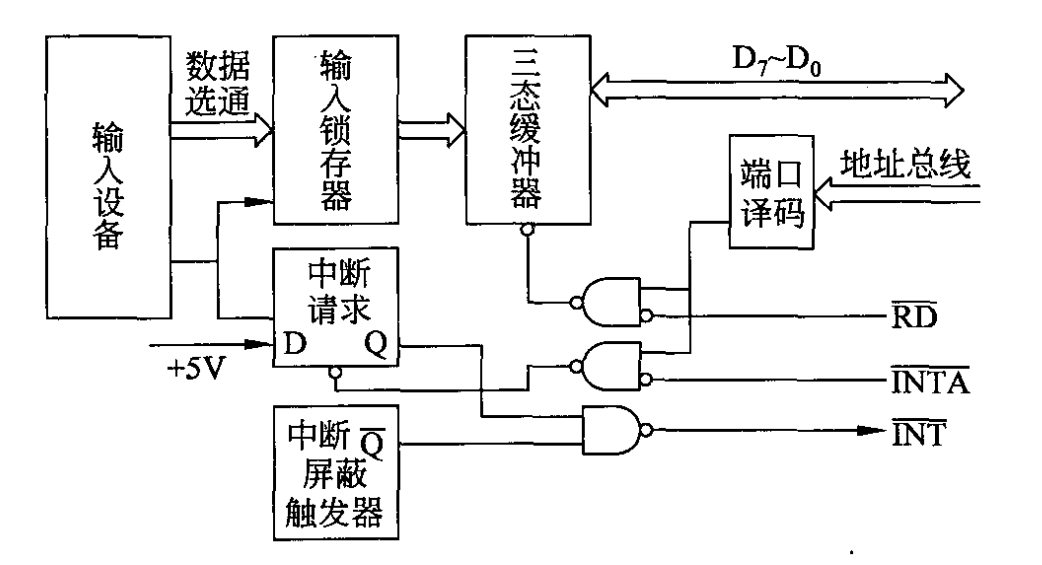
\includegraphics[scale=0.5]{1.PNG}
	\caption{中断方式输入的接口电路}
\end{figure}
\subsection{可屏蔽中断的响应和执行}
第一步接口发出中断请求信号,然后当前指令执行完以后,第二步CPU进行中断应答,也就是发出$\overline{\mathrm{INTA}}$信号,从引脚送到控制总线上去,第三步,中断响应信号的第二个负脉冲就被接口利用来打开三态门,把中断号通过数据总线送到CPU,第四步将当前标志寄存器的内容推入堆栈,第五步清除IF和TF,第六步查中断向量表,将中断号乘上4作为地址,前两个字节取出来给IP,后两个字节取出来给CS,所以CS和IP就指向中断子程序的入口,然后取指令执行。注意第八步STI开中断,主要是为了能够让其他中断能够嵌套它。
\begin{figure}[h]
	\centering
	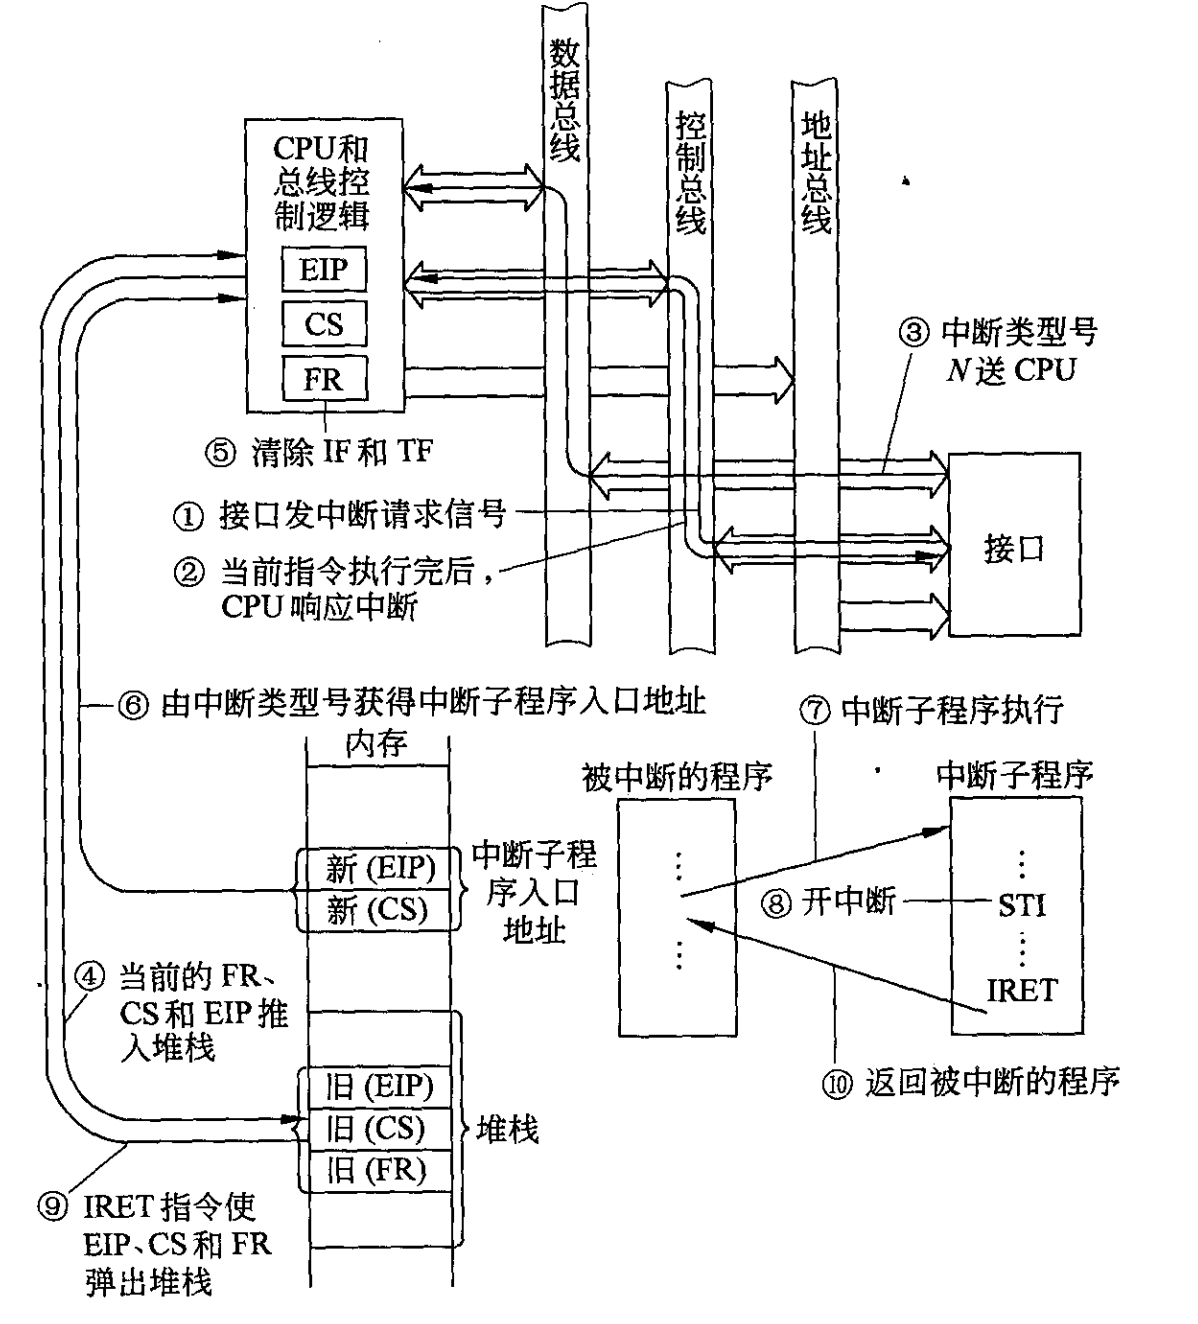
\includegraphics[scale=0.5]{2.PNG}
    \caption{可屏蔽中断的响应和执行}
\end{figure}
\subsection{中断优先级的解决}
从图3中可以看到,中断控制器中除中断优先级管理电路和中断请求锁存器外,还有中断类型寄存器,当前中断服务寄存器和中断屏蔽寄存器。\par
CPU的INTR引脚和$\overline{\mathrm{INTA}}$引脚连接中断控制器;另一方面,来自外设的I/O接口的中断请求信号并行地送到中断优先级管理电路,此管理电路为各中断请求信号分配优先级,比如最高的优先级分配给$IR_0$,下一个优先级分配给$IR_1$……,最低的优先级分配给$IR_7$等。当一个外部中断请求被中断优先级管理电路确定是当前级别最高的中断请求时,中断类型寄存器的最低3位的值(即对应与中断请求的序号)就会送到当前中断服务寄存器。此后,中断控制器向CPU发中断请求信号INTR,如中断允许标志为1,则CPU发出中断响应信号$\overline{\mathrm{INTA}}$,中断控制器在接到两个$\overline{\mathrm{INTA}}$的负脉冲之后,边疆中断类型号发给CPU。整个过程中,优先级较低的请求收到阻塞,知道通过程序中的指令或者由于中断处理程序执行完毕而引起当前中断服务寄存器的对应位清0,级别较低的中断请求才可能得到响应。
\begin{figure}[h]
	\centering
	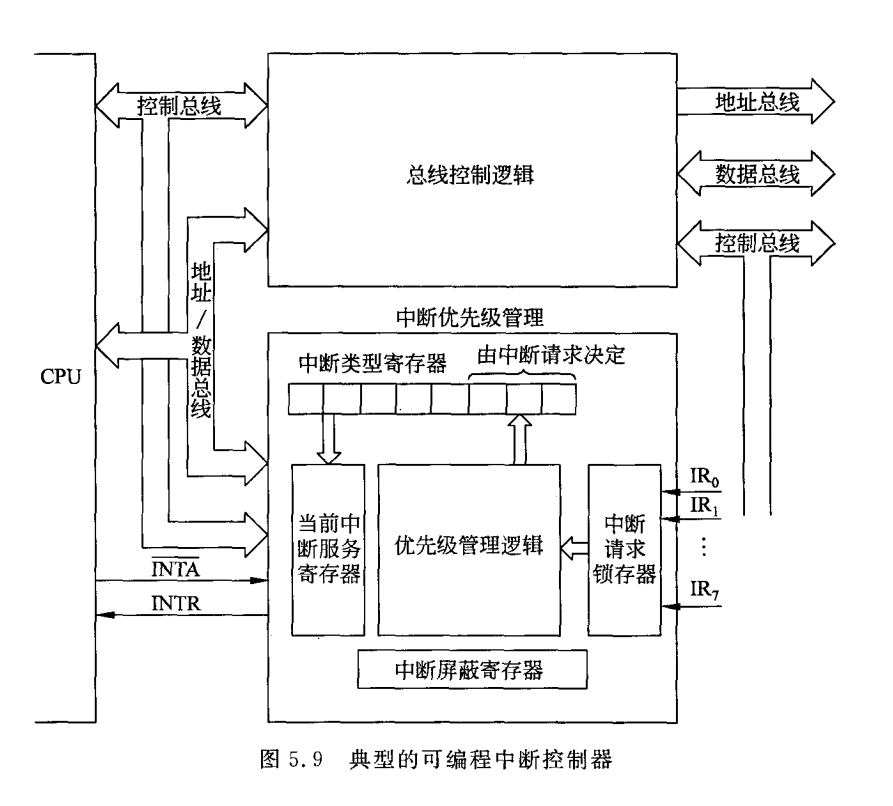
\includegraphics[scale=0.7]{3.PNG}
    \caption{典型的可编程中断控制器}
\end{figure}
\section{编程者如果用中断应该如何去做(以8086为例)}
\subsection{内中断}
\subsubsection{内中断的产生}
当CPU的内部有什么事情发生的时候,将产生需要马上处理的中断信息呢?对于8086CPU,当CPU内部有下面的情况发生的时候,将产生相应的中断信息。
\begin{itemize}
  \item 除法错误,比如div指令产生的除法溢出
  \item 单步执行
  \item 执行into指令
  \item 执行int指令
\end{itemize}
上述四种情况在8086CPU中的中断类型码依次为0,1,4和一个字节型类型数。
\subsubsection{中断过程的程序描述}
在前面我们用了文字表述中断过程,这里我们更简洁的描述一次
\begin{enumerate}[(1)]
  \item 取得中断类型码N
  \item pushf
  \item TF=0,IF=0
  \item push CS
  \item push IP
  \item (IP)=(N*4),(CS)=(N*4+2)
\end{enumerate}
在最后一步完成后,CPU开始执行程序员编写的中断处理程序
\subsubsection{内中断的程序实例}
例子:编写7ch的中断例程\par
功能:求一word型数据的平方\par
参数:(ax)=要计算的数据\par
返回值:dx、ax中存放结果的高16位和低16位\par
应用举例:求$2*3456^{2}$
\begin{lstlisting}
assume cs:code

code segment
    
    start:mov ax, 3456   ;(ax)=3456
    int 7ch              ;calculate the square of data in ax
    add ax, ax
    adc dx, dx           ;save result in dx:ax and twice it over
    mov ax, 4c00h
    int 21h
    
code ends    

end start    
\end{lstlisting}
\subsection{外中断}
之前我们讨论的都是CPU对于指令的执行。我们知道,CPU在计算机系统中,除了能够执行指令,进行运算以外,还能够对外部设备进行控制,接收他们的输入,对他们进行输出。接下来我们详细讨论外中断。
\subsubsection{外中断源}
外中断源可以分为两类:可屏蔽中断和不可屏蔽中断,几乎所有由外设引发的外中断,都是可屏蔽中断。当外设由需要处理的事件发生时,相关芯片向CPU发出可屏蔽中断信息。不可屏蔽中断是在系统中又必须紧急处理的紧急情况来通知CPU的信息。
\subsubsection{外中断的程序实例}
我们以键盘输入为例,编写int9中断例程。\par
编程:在屏幕中依次显示"a"-"z"\par
\begin{lstlisting}
assume cs:code
code segment
start: mov ax,0b800h
       mov es, ax
       mov ah, `'`a`'`
    s: mov es:[160*2+40*2], ah
       inc ah
       cmp ah, `'`z`'`
       jna s
       mov ax, 4c00h
       int 21h
code ends
end start
\end{lstlisting}
\section{结语}
由于笔者学识和经历有限, 因而对这个中断问题的探讨也只能提出个人较为粗浅的认识。在之后的仿真作业中会进一步的对所学知识进行学习和运用。
\begin{thebibliography}{1}

\bibitem{1}
微型计算机技术及其应用(第四版). 戴梅萼、史嘉权 . 清华大学出版社

\bibitem{2}
汇编语言(第三版). 王爽. 清华大学出版社


\end{thebibliography}
\end{document} 